% ragni-cas - a simple computer algebra system aimed at code generation and templating

% Disable review before sending
\documentclass[preprint, 12pt, a4paper]{elsarticle}

\usepackage[english]{babel}

\usepackage{amsmath}
\usepackage{amssymb}
\usepackage{pgf}
\usepackage[hidelinks]{hyperref}

\usepackage{lineno}
\usepackage{sty/tikz-uml}
\usetikzlibrary{arrows,automata}

% Code listing
\usepackage{xcolor,listings}
\lstdefinestyle{customruby}{
  belowcaptionskip=0.3\baselineskip,
  breaklines=true,
  frame=tb,
  xleftmargin=\parindent,
  language=Ruby,
  showstringspaces=false,
  basicstyle=\footnotesize\ttfamily\color{black},
  keywordstyle=\color{red!40!black},
  commentstyle=\color{gray},
  identifierstyle=\color{black},
  stringstyle=\color{green!40!black},
}
\lstloadlanguages{Ruby}
\lstset{style=customruby}

% !TEX root = ../Ragni2016.tex

\newcommand{\reviewB}[1]{{\color{blue} #1}\xspace}
\newcommand{\review}[1]{{#1}\xspace}

\newcommand{\Ruby}{\emph{Ruby}\xspace}
\newcommand{\Mruby}{\emph{mRuby}\xspace}
\newcommand{\Jruby}{\emph{JRuby}\xspace}
\newcommand{\ragnicas}{\emph{Mr.CAS}\xspace}

%% Library command
\newcommand{\Array}{\texttt{Ar\-ray}}
\newcommand{\Float}{\texttt{Flo\-at}}
\newcommand{\Fixnum}{\texttt{Fix\-num}}

\newcommand{\Namespace}{\texttt{::}}

\newcommand{\CAS}{\texttt{CAS}}
\newcommand{\CASOp}{\CAS\Namespace\texttt{Op\-}}
\newcommand{\CASBinaryOp}{\CAS\Namespace\texttt{Bi\-na\-ry\-Op}}
\newcommand{\CASNaryOp}{\CAS\Namespace\texttt{Nary\-Op}}

\newcommand{\CASExpression}{\CAS\Namespace\texttt{Con\-di\-tion}}

\newcommand{\CASSin}{\CAS\Namespace\texttt{Sin}}
\newcommand{\CASSum}{\CAS\Namespace\texttt{Sum}}
\newcommand{\CASDiff}{\CAS\Namespace\texttt{Diff}}

\newcommand{\CASVariable}{\CAS\Namespace\texttt{Va\-ria\-ble}}
\newcommand{\CASConstant}{\CAS\Namespace\texttt{Con\-stant}}
\newcommand{\CASFunction}{\CAS\Namespace\texttt{Func\-tion}}
\newcommand{\CASPiecewise}{\CAS\Namespace\texttt{Piece\-wise}}

\newcommand{\CASOpsimplify}{\CASOp\texttt{\#sim\-pli\-fy}}
\newcommand{\CASOpsubs}{\CASOp\texttt{\#subs}}
\newcommand{\CASOpdiff}{\CASOp\texttt{\#diff}}
\newcommand{\CASOpcall}{\CASOp\texttt{\#call}}


\journal{SoftwareX}

\begin{document}

%  ___            _              _   _
% | __| _ ___ _ _| |_ _ __  __ _| |_| |_ ___ _ _
% | _| '_/ _ \ ' \  _| '  \/ _` |  _|  _/ -_) '_|
% |_||_| \___/_||_\__|_|_|_\__,_|\__|\__\___|_|
\begin{frontmatter}

\title{\ragnicas~- A Pure \Ruby~Automatic Differentiation Library for Fast Prototyping of Interfaces}

\author[ragni]{Matteo Ragni}
\address[ragni]{Department of Industrial Engineering, University of Trento, 9, Sommarive, Povo di Trento, Italy}
\ead{matteo.ragni@unitn.it}

\begin{abstract}

Ca. 100 words

\end{abstract}

\begin{keyword}
CAS \sep{} code-generation \sep{} Ruby
%% PACS codes here, in the form: \PACS code \sep code
%% MSC codes here, in the form: \MSC code \sep code
%% or \MSC[2008] code \sep code (2000 is the default)
\end{keyword}

\end{frontmatter}

%% TODO: Disable line-numbers before sending
\linenumbers{}
%%

%% Body
% !TEX root = Ragni2016.tex

%  __  __     _   _          _   _
% |  \/  |___| |_(_)_ ____ _| |_(_)___ _ _
% | |\/| / _ \  _| \ V / _` |  _| / _ \ ' \
% |_|  |_\___/\__|_|\_/\__,_|\__|_\___/_||_|
\section{Motivation and significance}
\label{sec:motivation}

% Introduce the scientific background and the motivation for developing the software.
% Explain why the software is important, and describe the exact (scientific) problem(s) it solves.
% Indicate in what way the software has contributed (or how it will contribute in the future) to the
% process of scientific discovery; if available, this is to be supported by citing a research paper
% using the software.
% Provide a description of the experimental setting (how does the user use the software?).
% Introduce related work in literature (cite or list algorithms used, other software etc.).
\Ruby \cite{flanagan2008ruby}~is a purely object-oriented scripting language designed in the mid-1990s by Yukihiro Matsumoto, internationally standardized since 2012 as ISO/IEC 30170.

With the advent of the \emph{Internet of Things}, a compact version of the \Ruby interpreter called \Mruby (\emph{eMbedded Ruby})~\cite{tanaka2015mruby} has been published on \emph{GitHub} by Matsumoto, in 2014. The new interpreter is a lightweight implementation, aimed at both low power devices and PC, and complies with the standard\cite{iso30170}. \Mruby has a completely new API, and it is designed to be embedded in complex projects as a front-end interface---e.g., a numerical optimization suite may use \Mruby to for problem definition.

The \Ruby code-base exposes a large set of utilities in core and standard libraries, that can be furthermore expanded through third party libraries, or \emph{gems}. Among the large number of available gems, \Ruby still lacks an \textbf{automatic symbolic differentiation} (ASD)~\cite{tolsma1998computational} engine that handles basic computer algebra routines, compatible with all different \Ruby interpreters.

Nowadays \Ruby is mainly known thanks to the web-oriented \emph{Rails} framework, Its expressiveness and elegance though make it intriguing for use in the scientific/technical field. An ASD-capable gem would prove a foundamental step in this direction, including the support for flexible code generation for high-level software---e.g.,\ IPOPT~\cite{wachter2009ipopt, wachter2006}\@.

\ragnicas\footnote{Minimalistic Ruby Computer Algebra System} is a gem implemented in pure \Ruby that supports symbolic differentiation (SD) and some computer algebra operations~\cite{von2013modern}. The library aims at:
\begin{itemize}
  \item support rapid prototyping of numerical algorithms and code generation to different target languages;
  \item when dealing with mathematical models, support a clean and separate formulation of conditioning rules for numerical issues, in order to support more robust code generation;
  \item create a complete open-source CAS system for the standard \Ruby language, as a long-term effort.
\end{itemize}

Other CAS libraries for \Ruby are available:
\begin{description}
  \item [\emph{Rucas}~\cite{rucas}, \emph{Symbolic}~\cite{symbolic}]: milestone gems, yet at early stage and with discontinued development status. Both offer basic simplification routines, although they lack differentiation.
  \item [\emph{Symengine}~\cite{symengine}]: is a wrapper of the \emph{symengine} C++ library. The back-end library is very complete, but it is compatible only with the \emph{vanilla C} \Ruby interpreter and has several dependencies.
  At best of Author knowledge, at the moment it seems not working using the \Ruby 2.x interpreter.
%At the moment, the \emph{SciRuby}~\cite{sciruby} project reports the gem as broken, and removed it from its own codebase. From a direct test, when performing SD of an arbitrary function, the engine always returns \texttt{nil}.
\end{description}

In Section~\ref{sec:description}, \ragnicas container and tree structure is explained in detail and applied to basic CAS tasks. In Section~\ref{sec:examples}, two examples on how to use the library as code generator or as interface are described. Finally, the reasons behind the implementation and the long term desired impact are depicted in Section~\ref{sec:impact}. All code listings are available at \url{http://bit.ly/Mr_CAS_examples}.

% !TEX root = Ragni2016.tex

%  ___                 _      _   _
% |   \ ___ ___ __ _ _(_)_ __| |_(_)___ _ _
% | |) / -_|_-</ _| '_| | '_ \  _| / _ \ ' \
% |___/\___/__/\__|_| |_| .__/\__|_\___/_||_|
%                       |_|
\section{Software description}
\label{sec:description}

% Describe the software in as much as is necessary to establish a vocabulary needed to explain
% its impact.

%    _          _    _ _          _
%   /_\  _ _ __| |_ (_) |_ ___ __| |_ _  _ _ _ ___
%  / _ \| '_/ _| ' \| |  _/ -_) _|  _| || | '_/ -_)
% /_/ \_\_| \__|_||_|_|\__\___\__|\__|\_,_|_| \___|
\subsection{Software Architecture}
\label{sec:architecture}

% Give a short overview of the overall software architecture; provide a pictorial component overview
% or similar (if possible). If necessary provide implementation details.

\ragnicas~is an object oriented ASD gem that supports some computer algebra routines such as \emph{simplifications} and \emph{substitutions}. When gem is required, it overloads methods of \Fixnum~and \Float~classes, making them compatible with foundamental symbolic classes.

Each symbolic expression (or operation) is the instance of an object, that inherits from a common virtual ancestor: \CASOp. An operation encapsulates sub-operations recursively, building a linked tree, that is the mathematical equivalent of function composition:
\begin{equation}
\left( f \, \circ \, g \right)
\end{equation}

\begin{figure}[ht!]
\centering
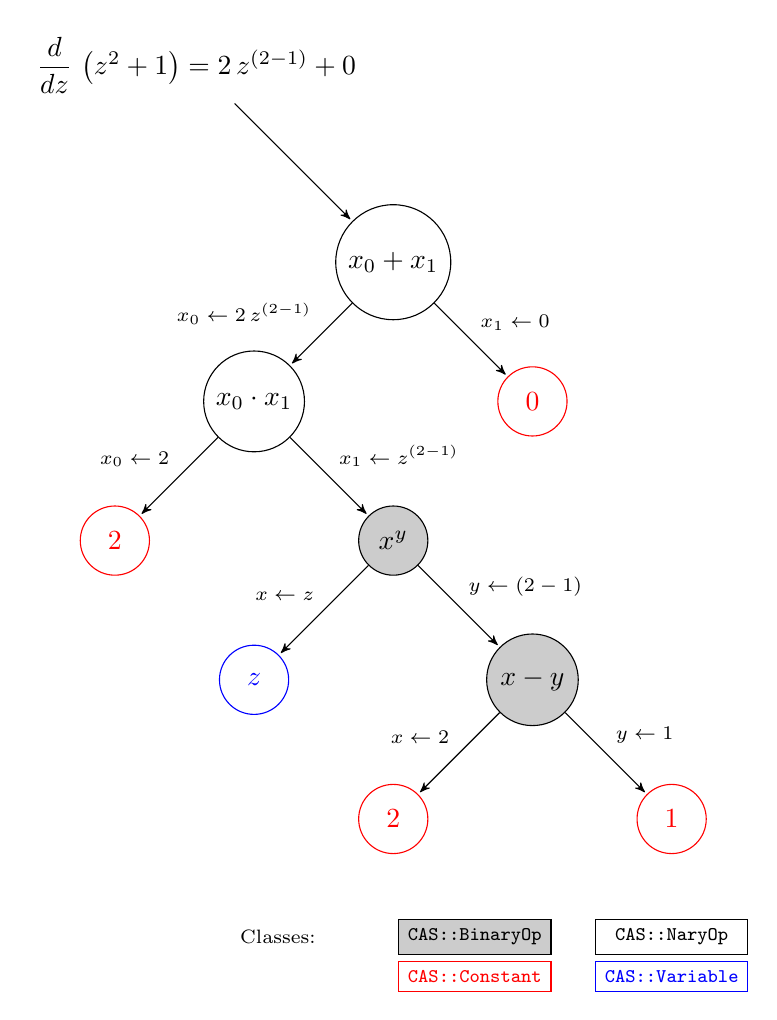
\begin{tikzpicture}[->,>=stealth',shorten >=1pt,auto,node distance=2.5cm]
  \tikzstyle{naryop}=[draw=black]
  \tikzstyle{constant}=[draw=red,text=red]
  \tikzstyle{variables}=[draw=blue,text=blue]
  \tikzstyle{binaryop}=[draw=black,fill=black!20]

  % Nodes
  \node[state]           (Sum)                          {$x_0 + x_1$};

  \node[state]           (Prod)  [below left of=Sum]    {$x_0 \cdot x_1$};
  \node[state,constant]  (Zero)  [below right of=Sum]   {$0$};

  \node[state,constant]  (Two)   [below left of=Prod]   {$2$};
  \node[state,binaryop]  (Pow)   [below right of=Prod]  {$x^y$};

  \node[state,variables] (X)     [below left of=Pow]    {$z$};
  \node[state,binaryop]  (Minus) [below right of=Pow]   {$x - y$};

  \node[state,constant]  (Two2)  [below left of=Minus]  {$2$};
  \node[state,constant]  (One)   [below right of=Minus] {$1$};

  % Legend
  \node[naryop]    (legend-Nary)   [below of=One,yshift=1cm] {\makebox[1.7cm]{\scriptsize\texttt{CAS::NaryOp}}};
  \node[binaryop]  (legend-Binary) [left of=legend-Nary]    {\makebox[1.7cm]{\scriptsize\texttt{CAS::BinaryOp}}};
  \node[variables] (legend-vars)   [below of=legend-Nary,yshift=2cm]     {\makebox[1.7cm]{\scriptsize\texttt{CAS::Variable}}};
  \node[constant]  (legend-const)  [left of=legend-vars]     {\makebox[1.7cm]{\scriptsize\texttt{CAS::Constant}}};
  \node (legendText) [left of=legend-Binary] {\scriptsize Classes:};

  % Origin
  \node (equation) [above of=Sum,xshift=-2.5cm] {$\dfrac{d}{dz}\,\left(z^2 + 1\right) = 2\,z^{(2 - 1)}+0$};

  \path (Sum)      edge node [anchor=south east] {\scriptsize $x_0 \leftarrow 2\,z^{(2 - 1)}$} (Prod)
                   edge node {\scriptsize $x_1 \leftarrow 0$}                                  (Zero)
        (Prod)     edge node [anchor=south east] {\scriptsize $x_0 \leftarrow 2$}              (Two)
                   edge node                     {\scriptsize $x_1 \leftarrow z^{(2-1)}$}      (Pow)
        (Pow)      edge node [anchor=south east] {\scriptsize $x \leftarrow z$}                (X)
                   edge node                     {\scriptsize $y \leftarrow (2 - 1)$}          (Minus)
        (Minus)    edge node [anchor=south east] {\scriptsize $x \leftarrow 2$ }               (Two2)
                   edge node                     {\scriptsize $y \leftarrow 1$ }               (One)
        (equation) edge                                                                        (Sum);
\end{tikzpicture}

\caption{\label{fig:graph}Tree of the expression derived in Listing~\ref{code:example-diff}}
\end{figure}

When a new operation is created, it is appended to the tree. The number of branches are determined by the parent container class of the current symbolic function. There are three possible containers:
\begin{description}
  \item[\CASOp] single sub-tree operation --- e.g.~$\sin(\cdot)$.
  \item[\CASBinaryOp] dual sub-tree operation --- e.g.~exponent $x^y$ --- that inherits from~\CASOp.
  \item[\CASNaryOp] operation with arbitrary number of sub-tree --- e.g.~sum $x_1 + \cdots + x_N$ --- that inherits from~\CASOp.
\end{description}
 Figure~\ref{fig:graph} contains a graphical representation. The different kind of containers allows to introduce some properties --- i.e.~\emph{associativity} and \emph{commutativity} for sums and multiplications~\cite{cohen2003computer}. Each container exposes the sub-tree as instance properties. Containers interfaces and inheritances are shown in Figure~\ref{fig:uml-container}. %TODO issue with image label

Terminal leafes of the graph are the classes \CASConstant, \CASVariable~and \CASFunction. The first models a simple numerical value, while the second represents an independent variable, that can be used to perform derivatives and evaluations, and the latter is a prototype of implicit functions. As for now, those leafes exemplify only real scalar expressions, with definition of complex, vectorial and matricial extensions as milestones for the next major release.

SD (\CASOpdiff) crosses the graph until it reaches ending nodes. A terminal node is the starting point for derivatives accumulation, the mathematical equivalent of the chain rule:
\begin{equation}
\left( f  \, \circ \, g \right)' \: = \:
\left( f' \, \circ \, g \right) \: g'
\end{equation}
The recursiveness is used also for simplifications (\CASOpsimplify), substitutions (\CASOpsubs), evaluations (\CASOpcall) and code generation.

\begin{figure}[ht!]
\centering
\begin{tikzpicture}
\umlclass[type=abstract]{CAS::Op}{
x : CAS::Op
}{
\umlvirt{ diff(CAS::Op) : CAS::Op } \\
\umlvirt{ subs(Hash) : CAS::Op    } \\
\umlvirt{ call(Hash) : Numeric } \\
\umlvirt{ simplify : CAS::Op      }
}

\umlclass[type=abstract,x=3,y=-5.5]{CAS::BinaryOp}{
x : CAS::Op \\
y : CAS::Op
}{}

\umlclass[type=abstract,x=3,y=-10.5]{CAS::NaryOp}{
x : Array
}{}

\umlemptyclass[x=8]{CAS::Sin}
\umlemptyclass[x=8,y=-2]{CAS::Log}
\umlsimpleclass[x=8,y=-3.5,draw=white]{...}

\umlemptyclass[x=8,y=-5.5]{CAS::Diff}
\umlemptyclass[x=8,y=-7.5]{CAS::Pow}
\umlsimpleclass[x=8,y=-9,draw=white]{...}

\umlemptyclass[x=8,y=-10.5]{CAS::Sum}
\umlemptyclass[x=8,y=-12.5]{CAS::Mul}
\umlsimpleclass[x=8,y=-14,draw=white]{...}


% Inheritance
\umlinherit[geometry=|-,anchor2=east]{CAS::BinaryOp}{CAS::Op}
\umlinherit[geometry=|-,anchor2=east]{CAS::NaryOp}{CAS::Op}

\umlinherit[geometry=--,anchor1=east,anchor2=east]{CAS::Sin}{CAS::Op}
\umlinherit[geometry=-|-,anchor1=east,anchor2=east]{CAS::Log}{CAS::Op}

\umlinherit[geometry=--,anchor1=east,anchor2=east]{CAS::Diff}{CAS::BinaryOp}
\umlinherit[geometry=-|-,anchor1=east,anchor2=east]{CAS::Pow}{CAS::BinaryOp}

\umlinherit[geometry=--,anchor1=east,anchor2=east]{CAS::Sum}{CAS::NaryOp}
\umlinherit[geometry=-|-,anchor1=east,anchor2=east]{CAS::Mul}{CAS::NaryOp}

\end{tikzpicture}

\caption{\label{fig:uml-container}Simplified version of classes interface and inheritance}
\end{figure}

%  ___             _   _               _ _ _   _
% | __|  _ _ _  __| |_(_)___ _ _  __ _| (_) |_(_)___ ___
% | _| || | ' \/ _|  _| / _ \ ' \/ _` | | |  _| / -_|_-<
% |_| \_,_|_||_\__|\__|_\___/_||_\__,_|_|_|\__|_\___/__/
\subsection{Software Functionalities}
\label{sec:functionalities}

\subsubsection{Software installation and prerequisites}

\emph{No additional dependencies are required}. The gem can be installed through \emph{rubygems.org} provider\footnote{\texttt{gem install Mr.CAS}}. Functionalities must be required runtime using the Kernel method: \texttt{require \'Mr.CAS\'}. All methods and classes are incapsulated in the module \texttt{CAS}.

\subsubsection{Basic Functionalities}
% Present the major functionalities of the software.
\textbf{SD} is performed with respect to independent variables (\CASVariable) through forward accumulation, even for implicit functions. The differentiation is done by the method \CASOpdiff, having a \CASVariable~as argument:

\noindent%
\lstinputlisting[caption={Differentiation example},label={code:example-diff}]{./scripts/listing_01.rb}

\textbf{Automatic differentiation} (AD) is included as plugin and exploits dual numbers~\cite{bartholomew2000automatic}. This differentiation strategy is useful in case of complex expressions, when explicit derivative's tree may exceed the call stack depth, that is platform dependent.

\textbf{Simplifications} are not executed automatically, after differentiations. Each node of the tree knows rules for simplify itself, and rules are called recursively, exactly like ASD.\@ Simplifications that require an \emph{heuristic expansion} of the subgraph --- i.e.\ some trigonometric identities --- are not defined for now, but can be easily achieved through \textbf{substitutions}:

\noindent%
\lstinputlisting[caption={Simplification example},label={code:example-simp}]{./scripts/listing_02.rb}

The tree is numerically \textbf{evaluated} when independent variables values are provided in a feed dictionary. The graph is reduced recursively to a single numeric value:

\noindent%
\lstinputlisting[caption={Tree evaluation example},label={code:example-call}]{./scripts/listing_03.rb}


Symbolic expressions can be used to create comparative expressions, that are stored in special container classes, modeled by the ancestor \CASExpression~--- e.g. $f(\cdot) \geq g(\cdot)$. This allow the definition of piecewise functions --- e.g. $\max(f(\cdot), g(\cdot))$.

\noindent%
\lstinputlisting[caption={Expressions and Piecewise functions},label={code:example-expr}]{./scripts/listing_04.rb}

\subsubsection{Metaprogramming and Code-Generation}

\ragnicas~is developed explicitly for \textbf{meta\-programming} and \textbf{generation of code}. Expressions can be exported as source code or used as prototypes for callable \emph{closures} (\texttt{Proc} objects):

\noindent%
\lstinputlisting[caption={Graph evaluation example},label={code:example-proc}]{./scripts/listing_05.rb}

Compiling a closure of a tree is like making its snapshot, thus any further manipulation of the expression do not update the callable object. This drawback is balanced by the faster execution time of a \texttt{Proc}: when a graph needs \emph{only to be evaluated} in a iterative algorithm, transforming it in a \emph{closure} reduces the execution time per iteration.

Code generation should be flexible enough to export expressions' trees in a user's target language. Generation methods for common languages are included in specific \textbf{plugins}. Users can furthemore expand exporting capabilites by writing specific exportation rules,  overriding method for existing plugin, or desining their own exporter:

\noindent%
\lstinputlisting[caption={Example of Ruby code generation plugin},label={code:example-exporting}]{./scripts/listing_06.rb}

% !TEX root = Ragni2016.tex

%  ___      _                _
% / __|_ _ (_)_ __ _ __  ___| |_ ___
% \__ \ ' \| | '_ \ '_ \/ -_)  _(_-<
% |___/_||_|_| .__/ .__/\___|\__/__/
%            |_|  |_|
%\subsection{Sample code snippets analysis (optional)}
%\label{sec:snippets}

% !TEX root = ../Ragni2016.tex

%  ___                     _
% | __|_ ____ _ _ __  _ __| |___ ___
% | _|\ \ / _` | '  \| '_ \ / -_|_-<
% |___/_\_\__,_|_|_|_| .__/_\___/__/
%                    |_|
\section{Illustrative Examples}
\label{sec:examples}

\subsection{Code Generation as C Library}
This example \review{shows how a \emph{user of \ragnicas} can export a mathematical model as a C library}. The \texttt{c-opt} plugin implements advanced features such as code optimization and generation of libraries.

The library \texttt{example} implements the model:
\begin{equation}
\label{eq:ex1model}
f(x, y) = x^y + g(x)\, \log(\sin(x^y))
\end{equation}
where the expression $g(x)$ belongs to a external object, declared as \texttt{g\_impl}, which interface is described in \texttt{g\_impl.h} header. \review{What should be noted is the corpus of the exported code}: the intermediate operation $x^y$ is evaluated once, even if appears twice in eq.~\ref{eq:ex1model}. The C function that implements $f(x,y)$ is declared with the token \texttt{f\_impl}. The exporter uses as default type \texttt{double} for variables and function returned values.

\noindent%
\lstinputlisting[caption={Calling optimized-C exporter for library generation},label={code:example-exporting-C-1}]{./scripts/example_01.rb}

Library created by \texttt{CLib} contains the code shown in Listing~\ref{code:c.ex.1}.

\noindent%
\begin{minipage}{.5\textwidth}
\lstinputlisting[style=customruby,language=C,caption={C Header}]{./scripts/source.h}
\end{minipage}\hfill
\begin{minipage}{.5\textwidth}
\lstinputlisting[style=customruby,language=C,caption={C Source},frame=tbl,label={code:c.ex.1}]{./scripts/source.c}
\end{minipage}

The function $g(x)$ models the following operation:
\begin{equation}
g(x) = (\sqrt{x + a} - \sqrt{x}) + \sqrt{\pi + x}
\end{equation}
and may suffer from \emph{catastrophic \review{numerical} cancellation}~\cite{higham2002accuracy} \review{when $x$ value is considerably greater than $a$}. The user \review{may decide to} specialize code generation rules for this particular expression, \review{stabilizing it} through rationalization. \review{Without modifying the actual model}, $g(x)$ the rationalization is inserted \review{into exportation rules}---cfr. Listing~\ref{code:example-exporting-C-2}---for differences of square roots\footnote{i.e.:
$\sqrt{\phi(\cdot)} - \sqrt{\psi(\cdot)} =
\dfrac{\phi(\cdot) - \psi(\cdot)}{\sqrt{\phi(\cdot)} + \sqrt{\psi(\cdot)}}$}.
\review{This rule is valid only for the current user script}. For more insight about \verb!__to_c! and \verb!__to_c_impl!\review{,} refer to the software manual.

\noindent%
\lstinputlisting[caption={Conditioning in exporting function},label={code:example-exporting-C-2}]{./scripts/example_02.rb}

It should be noted the separation between the \emph{model}---that does not contain \review{stabilization}---and the \emph{code generation rule}. For this particular case, the code generation rule in Listing~\ref{code:example-exporting-C-2} overloads the predefined one, in order to \review{obtain the conditioned code}. Obviously, the user can decide to apply directly the conditioning on the model itself\review{, but this may change the calculus behavior in further manipulation}.

\noindent%
\begin{minipage}{.5\textwidth}
\lstinputlisting[style=customruby,language=C,caption={\texttt{g\_impl} Header}]{./scripts/g_impl.h}
\end{minipage}\hfill
\begin{minipage}{.5\textwidth}
\lstinputlisting[style=customruby,language=C,caption={\texttt{g\_impl} Source},frame=tbl]{./scripts/g_impl.c}
\end{minipage}

\subsection{Using the module as interface}
As example, an implementation of an algorithm that estimates the \emph{order of convergence} for trapezoidal integration scheme~\cite{weideman2002numerical} is provided, using the symbolic differentiation as interface.

Given a function $f(x)$, the trapezoidal rule for primitive estimation for the interval $[a,\,b]$ is:
\begin{equation}
  I_{n}(a, b) = h\, \left( \dfrac{f(a) + f(b)}{2} +
    \sum\limits_{k = 1}^{n - 1}{f \left( a + k \,h \right)} \right)
\end{equation}
with $h = (b - a) / n $, where $n$ mediates the step size of the integration. When exact primitive $F(x)$ is known, approximation error is:
\begin{equation}
  E[n] = F(b) - F(a) - I_{n}(a, b)
\end{equation}
The error has an asymptotic expansion of the form:
\begin{equation}
  E[n] \propto C\,{n}^{-p}
\end{equation}
where $p$ is the convergence order. Using a different value for $n$, for example $2\,n$, the ratio~\ref{eq:error.ratio} takes the approximate vale:
\begin{equation}
  \label{eq:error.ratio}
  \dfrac{E[n]}{E[2\,n]} \approx 2^{p} \quad \rightarrow \quad p \approx \log_2 \left( \dfrac{E[n]}{E[2\,n]} \right)
\end{equation}
The Listings~\ref{code:example-integrate-ruby} and \ref{code:example-integrate-python} contain the implementation of the described procedure using the proposed gem and the well known \emph{Python}~\cite{van2011python} library \emph{SymPy}~\cite{christopher_smith_2016_47274}.

\noindent%
\begin{minipage}{.5\textwidth}
\lstinputlisting[style=customruby,caption={Ruby version},label={code:example-integrate-ruby}]{./scripts/example_03.rb}
\end{minipage}\hfill
\begin{minipage}{.5\textwidth}
\lstinputlisting[style=customruby,language=python,caption={Python version},frame=tbl,label={code:example-integrate-python}]{./scripts/example_03.py}
\end{minipage}

\review{
\subsection{ODE Solver with Taylor's series}

In this example, a solving step for a specific ordinary differential equation (ODE) using Taylor's series method~\cite{Butcher20081} is derived. Given an ODE in the form:
\begin{equation}
\label{eq:taylor.ode}
y'(x) = f\left(x, y(x)\right)
\end{equation}
the integration step with order $n$ has the form:
\begin{equation}
y(x + h) = y(x)  + h\,y'(x) + \dots + \dfrac{h^{n}}{n!} \, y^{(n)}(x) + E_{n}(x)
\end{equation}
where, obviously, it is possible to use equation~\ref{eq:taylor.ode}, which brings to the following recurrent identity:
\begin{equation}
{y}^{(i)}(x) =
\dfrac{\partial {y}^{(i-1)}(x)}{\partial x} +
\dfrac{\partial {y}^{(i-1)}(x)}{\partial y} {y'}(x)
\end{equation}
For this algorithm, three methods are defined. The first evaluates the factorial, the second evaluates the list of required derivatives, and the third returns the integration step in a symbolic form. The result of the third method is transformed in a C function. In this particular case, the ODE is $y' = x y$.
\lstinputlisting[caption={Generator for ODE integration step},label={code:example-ode}]{./scripts/listing_07.rb}
For the resulting C code, refer to the online version of the examples.

Other examples are available online\footnote{\url{http://bit.ly/Mr_CAS_examples}}:
\begin{enumerate*}[label=\emph{\alph*}.]
\item adding a user defined \CASOp~that implements the $\mathrm{sign}(\cdot)$ function with the appropriate optimized C generation rule;
\item exporting the operation as a continuous function through overloading or substitutions;
\item performing a symbolic Taylor's series;
\item writing an exporter for the \LaTeX{} language;
\item a Newton-Raphson algorithm using automatic differentiation plugin.
\end{enumerate*}
} % review

% !TEX root = Ragni2016.tex

%  ___                     _
% |_ _|_ __  _ __  __ _ __| |_
%  | || '  \| '_ \/ _` / _|  _|
% |___|_|_|_| .__/\__,_\__|\__|
%           |_|
\section{Impact}
\label{sec:impact}

% \textbf{This is the main section of the article and the reviewers weight the description here appropriately}
% Indicate in what way new research questions can be pursued as a result of the software (if any).
% Indicate in what way, and to what extent, the pursuit of existing research questions is improved (if so).
% Indicate in what way the software has changed the daily practice of its users (if so).
% Indicate how widespread the use of the software is within and outside the intended user group.
% Indicate in what way the software is used in commercial settings and/or how it led to the creation
% of spin-off companies (if so).
There are different complete CAS systems on the market, with complete solutions for analysis of analitical models. But exporting a model, for optimization or any other research activity, requires a lot of work, even with a good CAS software.

This library is a midpoint between a CAS and an AD library. It allows to manipulate expressions while mantaining the complete control on how the code is exported. Each rule is overloaded and applied runtime, without the need of compilation. Each user's model may include the mathematical description, code generation rules and high level logic that should be intrisic to such a rule --- e.g.~exporting gradients as \textbf{patterns} instead of matrices.

Our research group is including \texttt{Mr.CAS} in a solver for optimal control problem with indirect methods, as interface for problems' description~\cite{biral2016notes}.

As a long term ambitious impact, this library will become a complete CAS for \Ruby~language, filling the empty space reported by \emph{SciRuby} for symbolic math engines. This will require time, and the gem's MIT license allows everyone to contribute to the project.

% !TEX root = ../Ragni2016.tex

%   ___             _         _
%  / __|___ _ _  __| |_  _ __(_)___ _ _  ___
% | (__/ _ \ ' \/ _| | || (_-< / _ \ ' \(_-<
%  \___\___/_||_\__|_|\_,_/__/_\___/_||_/__/
\section{Conclusions}
\label{sec:conclusions}

% Set out the conclusion of this original software publication.
This work presents a pure \Ruby~library that implements a minimalistics CAS with
automatic and symbolic differentiation that is aimed at code generation and meta-programming.
Although at an early developing stage, \ragnicas~has promising feature, some of them
shown in Section~\ref{sec:examples}. Also, this is the only gem that implements
symbolic manipulation for this language.

Language features and lack of dependencies simplify the use of the module as interface, extending model definition
capabilities for numerical algorithms. All core functionalities and basic mathematics are defined, with the plan to include more features in next releases. Reopening a class guarantees a
\emph{liquid} behaviour, in which users are free to modify core methods at their needs.

Library is published in \emph{rubygems.org} repository and versioned on \emph{github.com}, under MIT license.
It can be included easily in projects and in inline interpreter, or installed as a standalone gem.


\section*{Acknowledgements}
\label{sec:acknowledgements}
This research did not receive any specific grant from funding agencies in the public, commercial, or not-for-profit sectors.

%% The Appendices part is started with the command \appendix;
%% appendix sections are then done as normal sections
%% \appendix

%% \section{}
%% \label{}

%  ___ _ _    _ _                         _
% | _ |_) |__| (_)___  __ _ _ _ __ _ _ __| |_ _  _
% | _ \ | '_ \ | / _ \/ _` | '_/ _` | '_ \ ' \ || |
% |___/_|_.__/_|_\___/\__, |_| \__,_| .__/_||_\_, |
%                     |___/         |_|       |__/
\bibliographystyle{elsarticle-num}
\bibliography{bib}


%\section*{Required Metadata}
%\label{}

% !TEX root = Ragni2016.tex

% __   __          _          _
% \ \ / /__ _ _ __(_)___ _ _ (_)_ _  __ _
%  \ V / -_) '_(_-< / _ \ ' \| | ' \/ _` |
%   \_/\___|_| /__/_\___/_||_|_|_||_\__, |
%                                   |___/
\section*{Current code version}
\label{sec:version-dev}

% Ancillary data table required for subversion of the codebase. Kindly replace examples in
% right column with the correct information about your current code, and leave the left column
% as it is.

\begin{table}[!h]
\begin{tabular}{|l|p{6.5cm}|p{6.5cm}|}
\hline
\textbf{Nr.} & \textbf{Code metadata description} & \textbf{Please fill in this column} \\
\hline
C1 & Current code version & 0.0.0 \\
\hline
C2 & Permanent link to code/repository used for this code version & \href{https://github.com/MatteoRagni/cas-rb}{github.com/MatteoRagni/cas-rb} \&
\href{https://rubygems.org/gems/ragni-cas}{rubygems.org/gems/ragni-cas} \\
\hline
C3 & Legal Code License   & MIT \\
\hline
C4 & Code versioning system used & \emph{git} (GitHub) \\
\hline
C5 & Software code languages, tools, and services used & \Ruby \\
\hline
C6 & Compilation requirements, operating environments & \Ruby $\geq 2.x$, \emph{pry} for testing console (optional) \\
\hline
C7 & If available Link to developer documentation/manual & \href{http://www.rubydoc.info/gems/ragni-cas}{rubydoc.info/gems/ragni-cas} \\
\hline
C8 & Support email for questions & \href{mailto:info@ragni.me}{info@ragni.me} \\
\hline
\end{tabular}
\caption{Code metadata (mandatory)}
\label{tab:code-metadata}
\end{table}

% \section*{Current executable software version}
% \label{sec:version-gem}
%
% % Ancillary data table required for sub version of the executable software: (x.1, x.2 etc.)
% % kindly replace examples in right column with the correct information about your executables,
% % and leave the left column as it is.
%
% \begin{table}[!h]
% \begin{tabular}{|l|p{6.5cm}|p{6.5cm}|}
% \hline
% \textbf{Nr.} & \textbf{(Executable) software metadata description} & \textbf{Please fill in this column} \\
% \hline
% S1 & Current software version & 0.0.0 \\
% \hline
% S2 & Permanent link to executables of this version  & \href{https://rubygems.org/gems/ragni-cas}{rubygems.org/gems/ragni-cas} \\
% \hline
% S3 & Legal Software License & MIT \\
% \hline
% S4 & Computing platforms/Operating Systems & x86, amd64, arm-hf, mips/Windows, Linux, OS-X \\
% \hline
% S5 & Installation requirements \& dependencies & \Ruby $\geq 2.x$, \emph{pry} gem for console (optional)\\
% \hline
% S6 & If available, link to user manual - if formally published include a reference to the publication in the reference list & Wiki not yet ready: \href{https://github.com/MatteoRagni/cas-rb/wiki/Welcome}{Project's Wiki} \\
% \hline
% S7 & Support email for questions & \href{mailt:info@ragni.me}{info@ragni.me} \\
% \hline
% \end{tabular}
% \caption{Software metadata (optional)}
% \label{}
% \end{table}

\end{document}
\endinput

%%
%% End of file `Ragni2016.tex'.
